\subsection{计算逻辑准确性测试}
Figure\ref{fig:sys.param}展示了测试计算逻辑模块的准确性时,系统输出的结果。
\begin{figure}[H]
\begin{center}
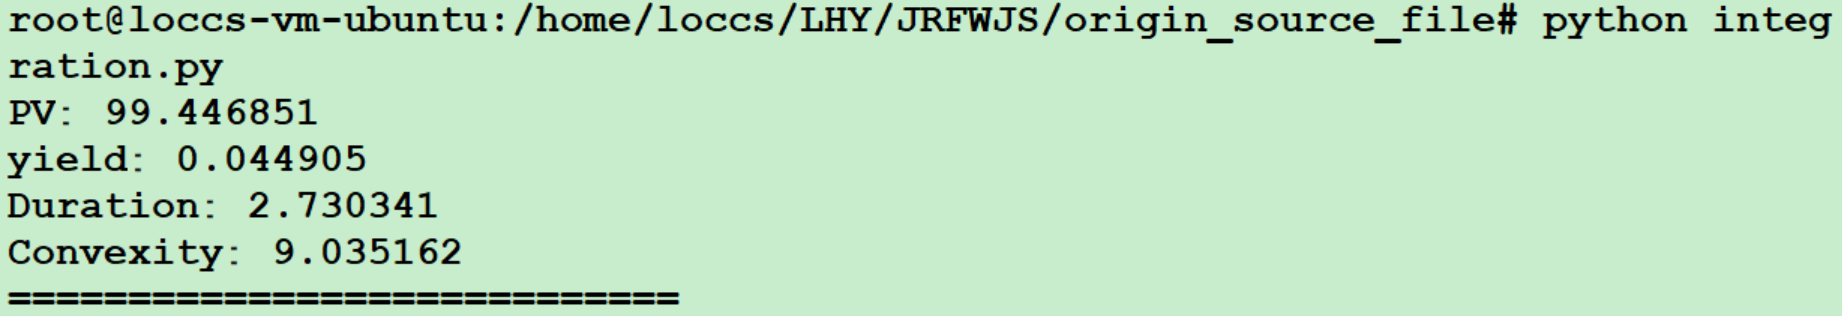
\includegraphics[width=16cm]{img//integration.PNG}
\caption{计算逻辑准确性测试}
\label{fig:sys.param}
\end{center}
\end{figure}


\subsection{自动测试结果}
Figure\ref{fig:sys.param}展示了使用自动测试程序测试本系统的准确性和性能时,自动测试程序输出的结果。
\begin{figure}[H]
\begin{center}
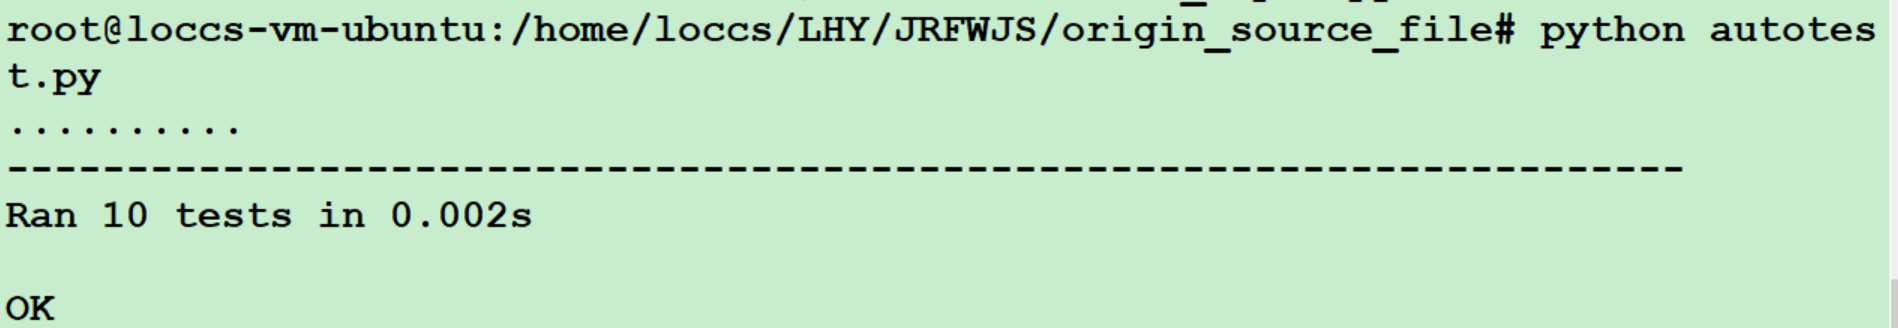
\includegraphics[width=16cm]{img//autotest.PNG}
\caption{自动测试结果}
\label{fig:sys.param}
\end{center}
\end{figure}


\subsection{调用多进程性能测试}
Figure\ref{fig:sys.param}展示了调用Python多进程时,系统输出的结果。
\begin{figure}[H]
\begin{center}
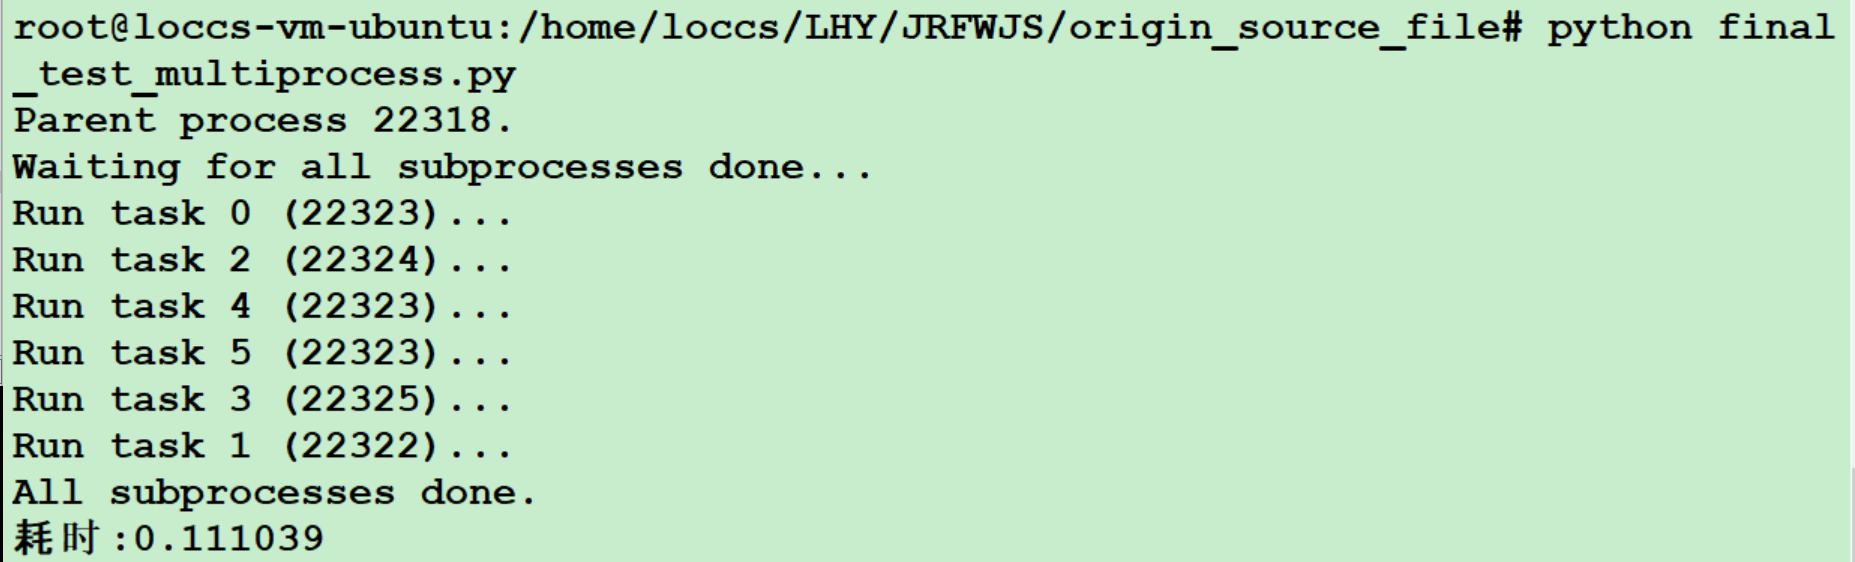
\includegraphics[width=16cm]{img//final_test_multiprocess.PNG}
\caption{调用多进程性能测试}
\label{fig:sys.param}
\end{center}
\end{figure}


\subsection{不使用并行计算}
Figure\ref{fig:sys.param}展示了不使用并行计算,运行用时103秒。
\begin{figure}[H]
\begin{center}
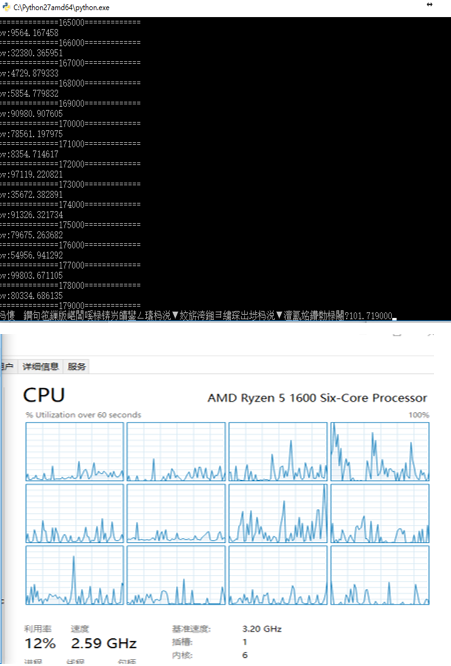
\includegraphics[width=16cm]{img//non_parallel.PNG}
\caption{不使用并行计算}
\label{fig:sys.param}
\end{center}
\end{figure}

\subsection{单机下并行计算}
Figure\ref{fig:sys.param}展示了单机并行百万级数据效果,用时11.83秒,效果不理想,因为文件io阻塞。
\begin{figure}[H]
\begin{center}
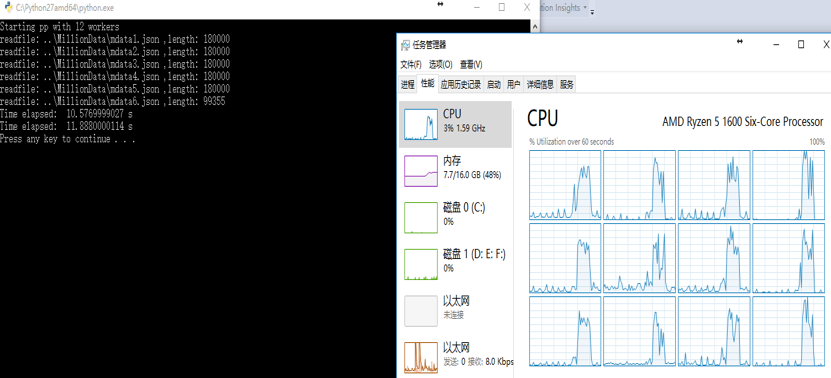
\includegraphics[width=16cm]{img//single_parallel.PNG}
\caption{单机下并行计算}
\label{fig:sys.param}
\end{center}
\end{figure}


\subsection{单机下并行计算的优化}
Figure\ref{fig:sys.param}展示了经过优化的单机并行百万级数据效果,用时10.63秒。
\begin{figure}[H]
\begin{center}
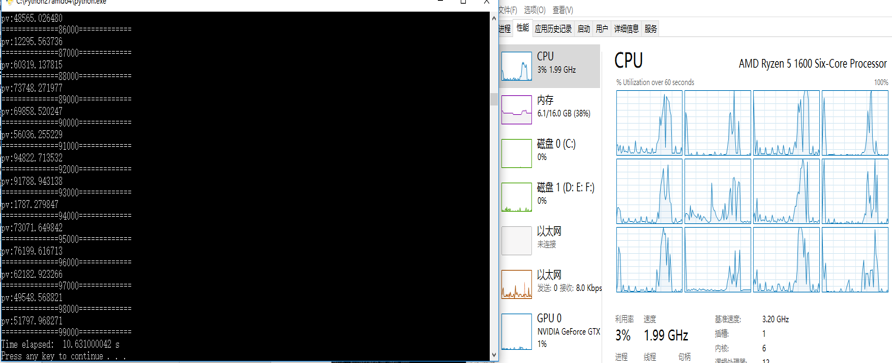
\includegraphics[width=16cm]{img//single_parallel_opt.PNG}
\caption{单机下并行计算的优化}
\label{fig:sys.param}
\end{center}
\end{figure}

\subsection{三百万数据测试}
Figure\ref{fig:sys.param}展示了三百万数据集下的测试结果。
\begin{figure}[H]
\begin{center}
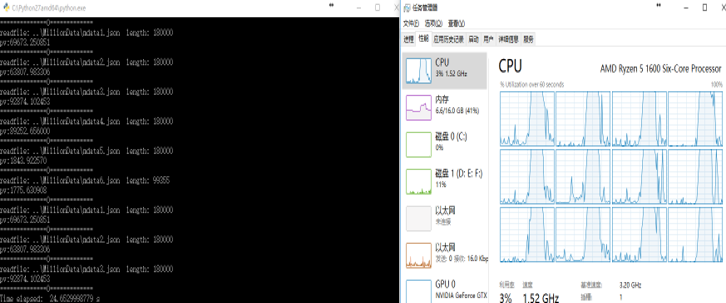
\includegraphics[width=16cm]{img//3million.PNG}
\caption{三百万数据测试}
\label{fig:sys.param}
\end{center}
\end{figure}

\subsection{分布式计算测试结果}
Figure\ref{fig:sys.param}展示了使用台式机+笔记本构成的集群下的测试结果。
\begin{figure}[H]
\begin{center}
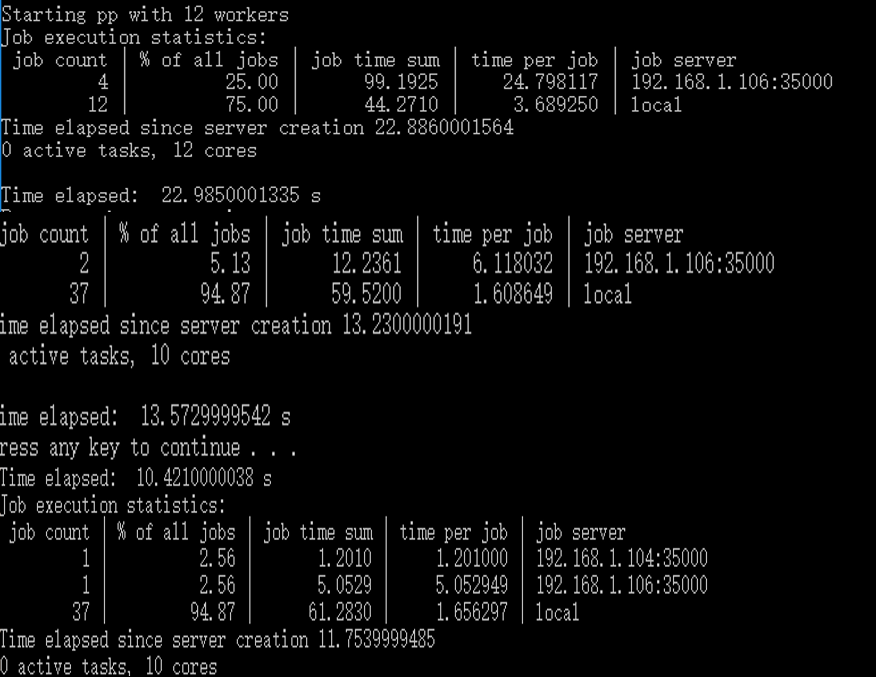
\includegraphics[width=16cm]{img//distribution.PNG}
\caption{分布式计算测试结果}
\label{fig:sys.param}
\end{center}
\end{figure}